\documentclass[journal]{IEEEtran}
\usepackage{graphicx,booktabs,xcolor,amsmath,amssymb,url,cite}
\usepackage{algorithm,algpseudocode}
\graphicspath{{../11_figures_tables/}{../../results/figures/}}
\providecommand{\tbd}{\textcolor{red}{\textbf{TBD}}}
\newcommand{\nAD}{36}
\newcommand{\nHC}{29}
\newcommand{\nFTD}{22}
\newcommand{\pctFemAD}{67\%}
\newcommand{\pctFemHC}{38\%}
\newcommand{\sexP}{\ensuremath{p=0.04}}
\newcommand{\epochsP}{\ensuremath{p=0.02}}
\newcommand{\ageP}{\ensuremath{p=0.38}}
\newcommand{\nDort}{200}
\newcommand{\nLemon}{70}
\newcommand{\dmMAE}{\ensuremath{9.2}}
\newcommand{\dmR}{\ensuremath{0.60}}
\newcommand{\hcMAE}{\ensuremath{7.4}}
\newcommand{\hcR}{\ensuremath{0.53}}
\newcommand{\hcRtwo}{\ensuremath{-1.9}}
\newcommand{\bagAD}{\ensuremath{-11.2}}
\newcommand{\bagADsd}{\ensuremath{14.2}}
\newcommand{\bagHC}{\ensuremath{0.0}}
\newcommand{\bagHCsd}{\ensuremath{9.4}}
\newcommand{\bagFTD}{\ensuremath{-2.2}}
\newcommand{\bagD}{\ensuremath{-0.91}}
\newcommand{\bagDci}{[\ensuremath{-1.50}, \ensuremath{-0.44}]}
\newcommand{\bagMwuP}{\ensuremath{p<0.001}}
\newcommand{\bagFTDd}{\ensuremath{-0.17}}
\newcommand{\bagFTDp}{\ensuremath{p=0.93}}
\newcommand{\bagADFTDd}{\ensuremath{-0.57}}
\newcommand{\bagADFTDp}{\ensuremath{p=0.04}}
\newcommand{\bagAUC}{\ensuremath{0.70}}
\newcommand{\origD}{\ensuremath{-0.93}}
\newcommand{\adjCoef}{\ensuremath{-10.3}}
\newcommand{\adjSE}{\ensuremath{3.0}}
\newcommand{\adjP}{\ensuremath{p=0.001}}
\newcommand{\adjECoef}{\ensuremath{-9.2}}
\newcommand{\adjEP}{\ensuremath{p=0.003}}
\newcommand{\resCoef}{\ensuremath{-9.1}}
\newcommand{\rawCoef}{\ensuremath{-9.1}}
\newcommand{\rawP}{\ensuremath{p<0.001}}
\newcommand{\hcFem}{\ensuremath{-5.5}}
\newcommand{\hcMale}{\ensuremath{3.5}}
\newcommand{\hcSexP}{\ensuremath{p=0.01}}
\newcommand{\stratFemD}{\ensuremath{-0.58}}
\newcommand{\stratFemP}{\ensuremath{p=0.12}}
\newcommand{\stratFemnAD}{24}
\newcommand{\stratFemnHC}{11}
\newcommand{\stratMaleD}{\ensuremath{-1.00}}
\newcommand{\stratMaleP}{\ensuremath{p=0.02}}
\newcommand{\stratMalenAD}{12}
\newcommand{\stratMalenHC}{18}
\newcommand{\epRho}{\ensuremath{0.31}}
\newcommand{\epP}{\ensuremath{p=0.07}}
\newcommand{\nStable}{12}
\newcommand{\nStableNeg}{12}
\newcommand{\nStableSig}{7}
\newcommand{\stableLo}{\ensuremath{-0.94}}
\newcommand{\stableHi}{\ensuremath{-0.27}}
\newcommand{\errTwenties}{\ensuremath{13.8}}
\newcommand{\errSixties}{\ensuremath{-7.2}}
\newcommand{\errSeventy}{\ensuremath{-15.8}}
\newcommand{\bagPermN}{500}
\newcommand{\bagPermP}{\ensuremath{p=0.002}}
\newcommand{\bagPermNullSD}{\ensuremath{0.28}}
\newcommand{\icaD}{\ensuremath{-0.70}}
\newcommand{\repD}{\ensuremath{-0.83}}
\newcommand{\repN}{513}
\newcommand{\lemADd}{\ensuremath{-0.58}}
\newcommand{\lemADp}{\ensuremath{p=0.007}}
\newcommand{\lemHCd}{\ensuremath{0.26}}
\newcommand{\lemHCp}{\ensuremath{p=0.18}}
\newcommand{\lemR}{\ensuremath{-0.03}}
\newcommand{\lemMAE}{\ensuremath{10.7}}
\newcommand{\ltwoD}{\ensuremath{-0.60}}
\newcommand{\ltwoP}{\ensuremath{p=0.01}}
\newcommand{\ltwoN}{270}
\newcommand{\thrDlo}{\ensuremath{-0.91}}
\newcommand{\thrDhi}{\ensuremath{-0.64}}
\newcommand{\thrAdjMaxP}{\ensuremath{p=0.02}}
\newcommand{\mmseRho}{\ensuremath{-0.08}}
\newcommand{\mmseP}{\ensuremath{p=0.62}}
\newcommand{\famAgree}{11 of 12}
\newcommand{\famSignP}{\ensuremath{p=0.006}}
\newcommand{\famAlphaD}{\ensuremath{0.65}}
\newcommand{\famAlphaP}{\ensuremath{p=0.002}}
\newcommand{\famSlowD}{\ensuremath{-0.97}}
\newcommand{\famSlowP}{\ensuremath{p<0.001}}
\newcommand{\famAperD}{\ensuremath{-0.84}}
\newcommand{\famAperP}{\ensuremath{p=0.002}}
\newcommand{\famFullD}{\ensuremath{-0.92}}
\newcommand{\normD}{\ensuremath{1.37}}
\newcommand{\normDci}{[\ensuremath{0.94}, \ensuremath{1.95}]}
\newcommand{\normAUC}{\ensuremath{0.83}}
\newcommand{\normAUCcv}{\ensuremath{0.83}}
\newcommand{\normFTDd}{\ensuremath{1.09}}
\newcommand{\normFTDp}{\ensuremath{p<0.001}}
\newcommand{\normADFTDp}{\ensuremath{p=0.36}}
\newcommand{\normAdjP}{\ensuremath{p<0.001}}
\newcommand{\cnnAUC}{\ensuremath{0.89}}
\newcommand{\cnnAcc}{82\%}
\newcommand{\cnnAUClo}{\ensuremath{0.86}}
\newcommand{\cnnAUChi}{\ensuremath{0.90}}
\newcommand{\cnnPrimAUC}{\ensuremath{0.86}}
\newcommand{\cnnPrimAUCci}{[\ensuremath{0.76}, \ensuremath{0.94}]}
\newcommand{\cnnPRAUC}{\ensuremath{0.89}}
\newcommand{\cnnBalAcc}{\ensuremath{0.80}}
\newcommand{\cnnSens}{\ensuremath{0.83}}
\newcommand{\cnnSpec}{\ensuremath{0.76}}
\newcommand{\cnnBrier}{\ensuremath{0.16}}
\newcommand{\cnnECE}{\ensuremath{0.10}}
\newcommand{\cnnCalSlope}{\ensuremath{1.28}}
\newcommand{\aucEEGNet}{\ensuremath{0.88}}
\newcommand{\aucRF}{\ensuremath{0.86}}
\newcommand{\aucSVM}{\ensuremath{0.85}}
\newcommand{\aucLR}{\ensuremath{0.84}}
\newcommand{\minHolmP}{\ensuremath{1.00}}
\newcommand{\holmText}{Holm-adjusted \ensuremath{p=1.00} for every comparison}
\newcommand{\cnnPermP}{\ensuremath{p=0.010}}
\newcommand{\cnnPermN}{100}
\newcommand{\subFemAUC}{\ensuremath{0.86}}
\newcommand{\subMaleAUC}{\ensuremath{0.89}}
\newcommand{\subAgeLo}{\ensuremath{0.77}}
\newcommand{\subAgeHi}{\ensuremath{0.89}}
\newcommand{\nestCnnAUC}{\ensuremath{0.87}}
\newcommand{\nestBagAUC}{\ensuremath{0.72}}
\newcommand{\nestCombAUC}{\ensuremath{0.87}}
\newcommand{\nestDiff}{\ensuremath{0.001}}
\newcommand{\nestDiffCI}{[\ensuremath{-0.07}, \ensuremath{0.07}]}
\newcommand{\nestDiffP}{\ensuremath{p=1.00}}
\newcommand{\nestBagP}{\ensuremath{p=0.002}}
\newcommand{\nestCnnAcc}{78\%}
\newcommand{\nestCombAcc}{74\%}
\newcommand{\occDelta}{\ensuremath{0.059}}
\newcommand{\occTheta}{\ensuremath{0.002}}
\newcommand{\occAlpha}{\ensuremath{0.018}}
\newcommand{\occBeta}{\ensuremath{0.108}}
\newcommand{\occGamma}{\ensuremath{0.014}}
\newcommand{\occOccipital}{\ensuremath{0.124}}
\newcommand{\occFrontal}{\ensuremath{0.114}}
\newcommand{\occTemporal}{\ensuremath{0.102}}
\newcommand{\occParietal}{\ensuremath{0.096}}
\newcommand{\occCentral}{\ensuremath{0.063}}
\newcommand{\gcStabLo}{\ensuremath{0.94}}
\newcommand{\gcStabHi}{\ensuremath{0.99}}
\newcommand{\gcTheta}{\ensuremath{1.25}}
\newcommand{\gcAlpha}{\ensuremath{1.29}}
\newcommand{\gcBeta}{\ensuremath{1.15}}
\newcommand{\gcDelta}{\ensuremath{0.77}}
\newcommand{\ablFull}{\ensuremath{0.89}}
\newcommand{\ablEight}{\ensuremath{0.85}}
\newcommand{\ablSixty}{\ensuremath{0.88}}
\newcommand{\ablMin}{\ensuremath{0.84}}
\newcommand{\ablSlow}{\ensuremath{0.85}}
\newcommand{\ablFast}{\ensuremath{0.87}}
\newcommand{\ablNoTime}{\ensuremath{0.84}}
\newcommand{\mcBalAcc}{63\%}
\newcommand{\mcAUC}{\ensuremath{0.78}}
\newcommand{\mcRFBalAcc}{56\%}

\makeatletter\newcommand{\tableinput}[1]{\@@input generated/#1 }\makeatother

\begin{document}

\title{Older or Younger? The Sign of the EEG Brain-Age Gap in Alzheimer's Disease Depends on the Spectral Features: A Leakage-Audited Normative Analysis}

\author{Aayush~Soni, Aamal~Magdum, Afreen~Anz, and~Aparna~Sankar%
\thanks{The authors are with the Department of Computer Science and Engineering, B.\,M.\,S. College of Engineering, Bengaluru, India.}}

\markboth{}{Soni \MakeLowercase{\textit{et al.}}: The sign of the EEG brain-age gap in Alzheimer's disease}
\maketitle

% =====================================================================
\begin{abstract}
\emph{Background:} EEG brain-age models trained on healthy adults are expected to show ``accelerated aging'' in neurodegeneration, and alpha-band EEG studies report positive brain-age gaps (BAG) in Alzheimer's disease (AD). We tested this expectation with a full-spectrum resting-state model under an audited, leakage-controlled protocol.
\emph{Methods:} A ridge brain-age model was trained on healthy adults (Dortmund Vital Study, $n=\nDort{}$, 20--70 years) and transferred to a clinical cohort (OpenNeuro ds004504: \nAD{} AD, \nHC{} healthy controls [HC], \nFTD{} frontotemporal dementia [FTD]). Patients were never used for training, harmonization, bias correction or model selection. We report leave-one-HC-out bias correction, nested model selection, age/sex adjustment, a permutation test that retrains the model ($N=\bagPermN{}$), an external healthy cohort (MPI-LEMON, $n=\nLemon{}$), a pre-registered feature-family analysis and a multivariate normative-deviation model. A CWT-scalogram CNN and four baselines were evaluated on identical subject-level folds, with nested stacking and occlusion-tested Grad-CAM.
\emph{Results:} The full-spectrum BAG was negative in AD ($d=\bagD{}$, 95\% CI \bagDci{}; age- and sex-adjusted difference \adjCoef{} years, \adjP{}; permutation \bagPermP{}). It was absent in FTD ($d=\bagFTDd{}$) and not shown by healthy older adults from an independent site. The sign depended on the features: alpha-only models made AD look older ($d=\famAlphaD{}$), slow-wave and aperiodic models made it look younger ($d=\famSlowD{}$, \famAperD{}), and \famAgree{} single-family models followed a pre-registered direction prediction (sign test \famSignP{}). A multivariate normative-deviation score separated AD from HC better than BAG (AUC \normAUC{} vs.\ \bagAUC{}) but also deviated in FTD. The CNN reached AUC \cnnAUC{} (three seeds), statistically indistinguishable from spectral baselines and EEGNet. BAG added no information to the CNN in nested stacking (\nestDiffP{}). Grad-CAM was stable across seeds, but occlusion did not confirm its emphasis on theta.
\emph{Conclusion:} The direction of the EEG brain-age gap in AD is a property of the feature set, not of the disease. AD EEG is better described as a multivariate deviation from normative aging than as accelerated or delayed aging. Validation in an independent AD cohort is needed.
\end{abstract}

\begin{IEEEkeywords}
Alzheimer's disease, electroencephalography, brain age, normative modeling, data leakage, explainable AI, convolutional neural network
\end{IEEEkeywords}

% =====================================================================
\section{Introduction}
\IEEEPARstart{R}{esting-state} EEG is an inexpensive, scalable candidate for Alzheimer's disease (AD) screening. AD is characterized by EEG ``slowing'': delta and theta activity increase, alpha and beta activity decrease, and the alpha peak frequency moves lower~\cite{jeong2004,babiloni2020}. Brain-age models trained on healthy people provide a normative alternative to patient-trained classifiers. The brain-age gap (BAG, predicted minus chronological age) is usually interpreted as accelerated aging~\cite{cole2017,franke2019}. For EEG, positive gaps in dementia have been reported from sleep recordings~\cite{ye2020} and, recently, from alpha-band resting-state activity in a large multi-site cohort~\cite{otero2026}.

The accelerated-aging interpretation assumes that disease moves the EEG \emph{along} the healthy-aging trajectory. Many spectral features change in healthy aging, however, and AD need not change all of them in the same direction. If it does not, the sign of an EEG brain-age gap would depend on which features the age model uses. Small clinical EEG cohorts are also vulnerable to leakage and analytic flexibility~\cite{brookshire2024,delpup2025,varoquaux2018}.

We therefore asked four questions under an audited, leakage-controlled protocol. (Q1) What is the sign of a full-spectrum resting-state BAG in AD, and does it survive leakage control, covariates and an external healthy site? (Q2) Does the sign depend on the spectral features of the age model, as predicted from feature-wise aging and disease directions? (Q3) Is a multivariate normative-deviation score more informative than a scalar BAG? (Q4) How does an explainable CWT-scalogram CNN compare with baselines, and do BAG or Grad-CAM add reliable information?

Our contributions are:
(i) a full-spectrum BAG that is robustly negative in AD under extensive leakage control;
(ii) a pre-registered demonstration that the BAG sign is feature-dependent, which reconciles our result with positive alpha-based gaps;
(iii) evidence that a multivariate normative-deviation score outperforms the scalar BAG but is not AD-specific;
(iv) an honest benchmark of an explainable CNN, including nested stacking and occlusion tests of Grad-CAM.

% =====================================================================
\section{Related Work}
\emph{EEG brain age in dementia.} Sleep-EEG brain age rises from non-demented to demented groups~\cite{ye2020}; see also~\cite{sun2019}. Otero et al.\ trained an alpha-only, source-space Elastic Net on healthy adults from ten countries and found older-appearing EEG in MCI, AD and behavioural-variant FTD, with modest effects~\cite{otero2026}. Resting-state EEG brain age in healthy populations has been benchmarked~\cite{alzoubi2018,engemann2022}. Bias correction is essential~\cite{delange2020}.

\emph{EEG classification of AD on ds004504.} The dataset authors reported 78.5\% accuracy for AD vs.\ controls with decision trees while comparing validation schemes~\cite{miltiadous2021}, and 83.3\% accuracy for AD vs.\ controls with leave-one-subject-out validation using DICE-net~\cite{miltiadous2023dice}. Deep EEG models more broadly are reviewed in~\cite{craik2019,roy2019}; EEGNet is a standard compact baseline~\cite{eegnet}.

\emph{Leakage and explainability.} Segment-level splits strongly inflate EEG deep-learning accuracy, including for AD~\cite{brookshire2024}, and subject-based cross-validation is required for cross-subject claims~\cite{delpup2025}. Grad-CAM~\cite{gradcam} attributions are widely used on EEG time--frequency images but are rarely tested for faithfulness.

% =====================================================================
\section{Materials and Methods}
\subsection{Cohorts}
\emph{Clinical:} OpenNeuro ds004504~\cite{miltiadous2023}: eyes-closed resting EEG, 19 channels (10--20), 500\,Hz, with MMSE scores. After preprocessing there were \nAD{} AD, \nHC{} HC and \nFTD{} FTD subjects; one FTD recording failed artifact screening. AD and HC did not differ in age (\ageP{}), but differed in sex (AD \pctFemAD{} vs.\ HC \pctFemHC{} female, \sexP{}) and in the number of clean epochs (\epochsP{}). Both variables are therefore used as covariates. There are no MCI subjects. \emph{Healthy training:} Dortmund Vital Study (OpenNeuro ds005385)~\cite{gajewski2022}; baseline eyes-closed pre-task recordings; age-stratified sample, $n=\nDort{}$, 20--70 years. \emph{External healthy:} MPI-LEMON older adults (5-year age bins, 55--80), eyes-closed blocks only, $n=\nLemon{}$, with an analysis plan committed to version control before processing.

\subsection{Preprocessing and features}
One function processes all data with MNE-Python~\cite{mne}. It selects 19 channels in a fixed order (10--10 names mapped to 10--20), applies an average reference, a 0.5--45\,Hz zero-phase FIR filter and resampling to 250\,Hz, and cuts 4\,s epochs with 2\,s overlap. Epochs whose peak-to-peak amplitude exceeds 150\,$\mu$V or falls below 1\,$\mu$V are rejected. Per channel we compute log absolute and relative delta, theta, alpha and beta power; alpha peak frequency; log theta/alpha ratio; and the aperiodic exponent and offset (FOOOF~\cite{fooof}). This gives 12 feature families $\times$ 19 channels = 228 features. A regional version (5 regions, 60 features) is used for the normative model.

\subsection{Brain-age model, bias correction and leakage control}
A ridge regressor (standardized features, inner-CV regularization) predicts age. Clinical HC are added to training with leave-one-HC-out prediction (strategy chosen from four candidates by nested leave-one-HC-out selection; patients are never involved). Bias is corrected with $\tilde y=(\hat y-b)/a$, where $(a,b)$ are fitted on out-of-fold HC predictions \emph{excluding the subject being corrected}, and $\mathrm{BAG}=\tilde y-y$~\cite{delange2020}. A residual correction ($\hat y-(ay+b)$) and an uncorrected gap with covariates are reported as alternatives. Group effects are tested with Cohen's $d$ (bootstrap CI), Mann--Whitney tests and OLS adjusting for age, sex and epoch count. A permutation test permutes AD/HC labels and \emph{retrains} the label-dependent model each time ($N=\bagPermN{}$). Automated guards assert that training and test subjects never overlap and that no AD or FTD subject enters training (\texttt{src/q1/guards.py}; 12 unit tests).

\subsection{Feature-family analysis (pre-registered)}
After reading~\cite{otero2026}, and before running the analysis (version-controlled commit), we hypothesized that a single-family age model makes AD look older if the family changes in the same direction in healthy aging and in AD, and younger otherwise. The predicted direction is $\mathrm{sign}(r_\mathrm{age,healthy}\cdot d_\mathrm{AD-HC})$. We trained the same pipeline on each of the 12 families and on alpha, slow-wave and aperiodic sets. Directions use the residual correction, because single-family models can have small or negative bias slopes.

\subsection{Normative-deviation model}
For each regional feature, a healthy-only reference model ($\text{feature}\sim\text{age}+\text{age}^2+\text{site}$) is fitted on Dortmund plus clinical HC. Each HC is scored with a reference fitted without that subject. Residual $z$-scores are summarized by a Mahalanobis distance (Ledoit--Wolf covariance).

\subsection{Classifiers and evaluation}
\emph{CWT-CNN:} Morlet scalograms (1--40\,Hz, 40 log-spaced frequencies, 64 time bins, $\le150$ epochs per subject; input $19\times40\times64$). A three-block CNN ($\approx$17k parameters) is trained with class-weighted cross-entropy and early stopping on validation \emph{subjects} from the training side. Subject probability is the mean over epochs. \emph{Baselines} on identical subject-level 10-fold splits: logistic regression, RBF-SVM and random forest on spectral features (inner-CV tuning), and EEGNet~\cite{eegnet}. \emph{Stacking} is fully nested (Algorithm~\ref{alg:nest}). \emph{Metrics:} AUC, PR-AUC, balanced accuracy, sensitivity, specificity, Brier score and expected calibration error, with 2000-sample bootstrap CIs; Holm-corrected paired bootstrap comparisons; a CNN permutation test that re-runs the full CV~\cite{ojala2010}. \emph{Explainability:} Grad-CAM~\cite{gradcam} out-of-fold for three seeds, plus occlusion. Each fold model re-scores its untouched test subjects with one band or scalp region set to the training mean.

\begin{algorithm}[t]
\caption{Fully nested stacking (outer fold $k$)}
\label{alg:nest}
\begin{algorithmic}[1]
\Require outer-train subjects $T$, outer-test subjects $E$ (disjoint)
\State inner 5-fold CV of the CNN within $T$ $\rightarrow$ out-of-fold $P_\mathrm{CNN}$ for $T$
\State train the CNN on $T$ (validation split inside $T$) $\rightarrow$ $P_\mathrm{CNN}$ for $E$
\State age model on Dortmund + HC$\in T$ (HC predicted leave-one-out); $E$ never trained on
\State bias correction from HC$\in T$; BAG for $T$ and $E$
\State fit logistic meta-model on $[\mathrm{logit}\,P_\mathrm{CNN},\mathrm{BAG}]$ of $T$; predict $E$
\end{algorithmic}
\end{algorithm}

% =====================================================================
\section{Results}
\subsection{Q1: The full-spectrum BAG is negative in AD}
On the healthy cohort the model reached MAE \dmMAE{} years ($r=\dmR{}$) in 10-fold CV. It showed the expected regression to the mean (mean signed error \errTwenties{} years in the 20s, \errSixties{} in the 60s and \errSeventy{} at 70). On clinical HC the out-of-fold MAE was \hcMAE{} years ($r=\hcR{}$; $R^2=\hcRtwo{}$, uninformative for a 57--78-year range). With leakage-free correction the BAG was $\bagHC{}\pm\bagHCsd{}$ years in HC, $\bagAD{}\pm\bagADsd{}$ in AD and \bagFTD{} in FTD. AD differed from HC ($d=\bagD{}$, \bagDci{}, Mann--Whitney \bagMwuP{}) and from FTD ($d=\bagADFTDd{}$, \bagADFTDp{}); FTD did not differ from HC ($d=\bagFTDd{}$, \bagFTDp{}). Table~\ref{tab:audit} and Fig.~\ref{fig:audit} show that the leakage corrections changed the effect minimally (originally reported $d=\origD{}$). Adjusting for age and sex gave \adjCoef{} years (SE \adjSE{}, \adjP{}), and adding epoch count gave \adjECoef{} years (\adjEP{}). Residual and uncorrected gaps gave \resCoef{} and \rawCoef{} years (\rawP{}). The retrained permutation test gave \bagPermP{} (null SD of $d$ \bagPermNullSD{}). All \nStable{} numerically stable model configurations were negative ($d$ \stableLo{} to \stableHi{}), and \nStableSig{} remained significant after age/sex adjustment. The effect persisted on ICA-cleaned recordings ($d=\icaD{}$), with \repN{} healthy training subjects ($d=\repD{}$), with a 20--80-year normative set including LEMON ($d=\ltwoD{}$, \ltwoP{}) and across artifact thresholds of 100--200\,$\mu$V ($d$ \thrDlo{} to \thrDhi{}; all age/sex-adjusted $p\leq$ \thrAdjMaxP{}). The magnitude was threshold-sensitive: the pre-specified 150\,$\mu$V threshold gave the largest effect. Healthy LEMON adults scored with the unchanged model did not differ from clinical HC ($d=\lemHCd{}$, \lemHCp{}), whereas AD differed from them ($d=\lemADd{}$, \lemADp{}). Within LEMON, predictions did not track age ($r=\lemR{}$). Within HC, women had lower BAG than men (\hcFem{} vs.\ \hcMale{} years, \hcSexP{}). Stratified by sex, the AD effect was present in men ($d=\stratMaleD{}$, \stratMaleP{}; \stratMalenAD{} AD vs.\ \stratMalenHC{} HC) and in the same direction but not significant in women ($d=\stratFemD{}$, \stratFemP{}; \stratFemnAD{} vs.\ \stratFemnHC{}). BAG was not associated with MMSE in AD ($\rho=\mmseRho{}$, \mmseP{}).

\begin{table}[t]
\centering
\caption{AD$-$HC brain-age effect under the leakage and bias-correction audit}
\label{tab:audit}
\scriptsize\setlength{\tabcolsep}{2pt}
\begin{tabular}{p{3.5cm}cc}
\toprule
Analysis & Cohen's $d$ [95\% CI] & MWU \\
\midrule
\tableinput{table_audit.tex}
\bottomrule
\end{tabular}
\end{table}

\begin{figure}[t]
\centering
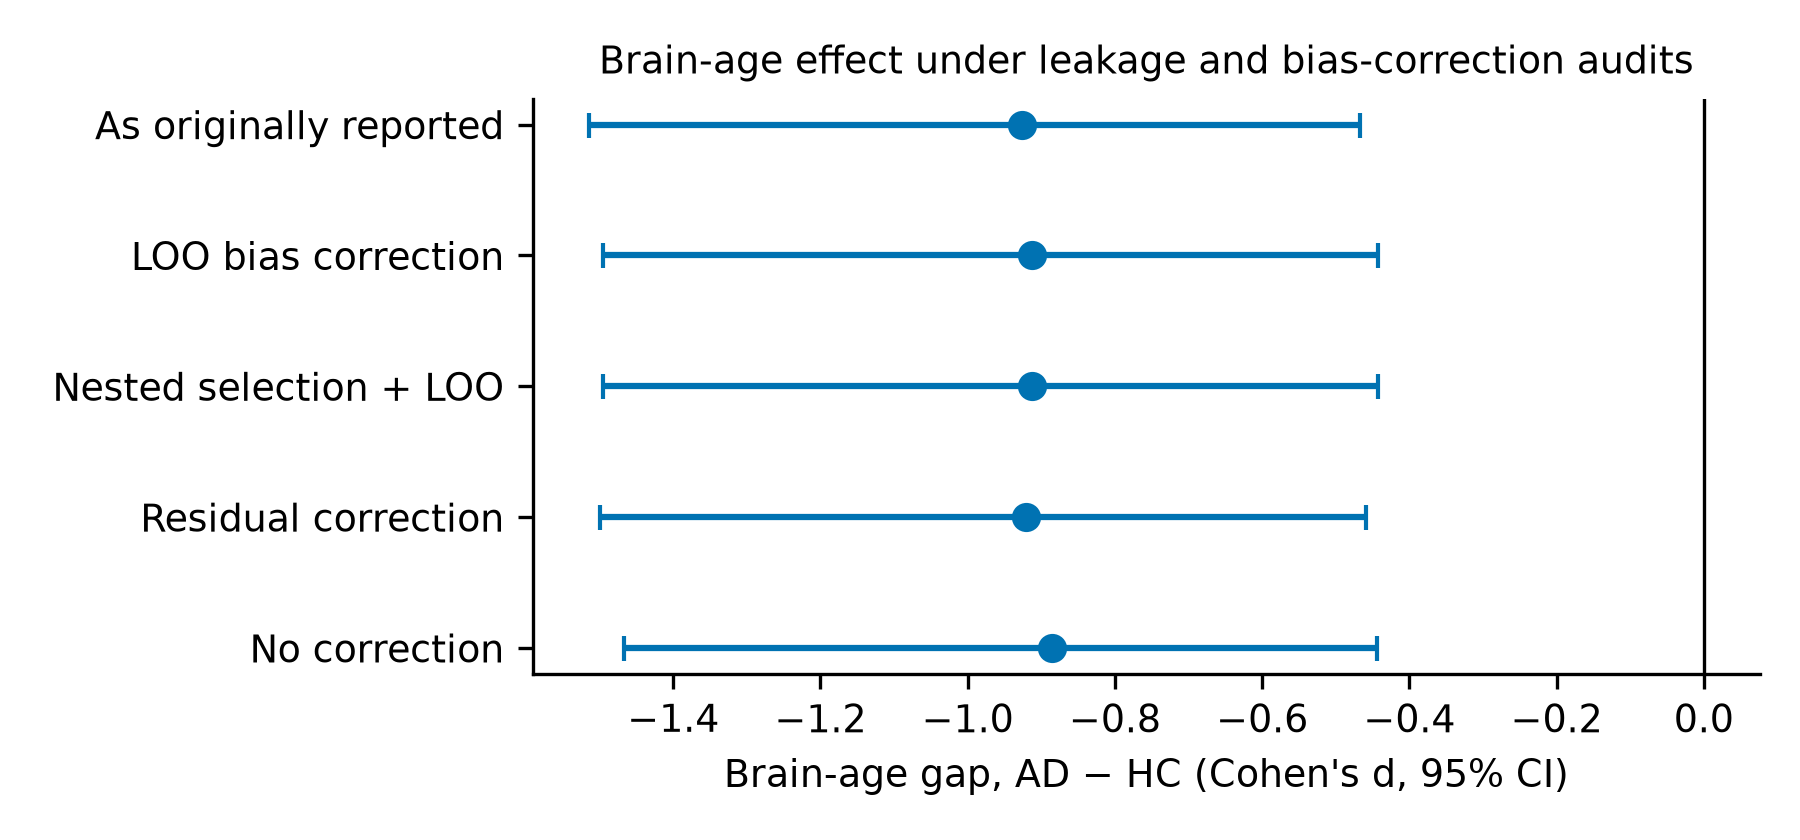
\includegraphics[width=0.95\columnwidth]{fig_brainage_audit.png}
\caption{Brain-age effect (AD$-$HC) under leakage and bias-correction variants.}
\label{fig:audit}
\end{figure}

\subsection{Q2: The sign of the BAG depends on the features}
\famAgree{} single-family models followed the pre-registered direction (Table~\ref{tab:fam}, Fig.~\ref{fig:fam}; sign test \famSignP{}). An alpha-only model made AD look \emph{older} ($d=\famAlphaD{}$, \famAlphaP{}), qualitatively reproducing alpha-based positive gaps~\cite{otero2026}. Slow-wave and aperiodic models made AD look younger ($d=\famSlowD{}$ and \famAperD{}). The full-spectrum model, dominated by these families, was negative ($d=\famFullD{}$). The single mismatch, the theta/alpha ratio, was not significant.

\begin{table}[t]
\centering
\caption{Single-family brain-age models: predicted vs.\ observed AD direction}
\label{tab:fam}
\scriptsize\setlength{\tabcolsep}{2.5pt}
\begin{tabular}{lcccc}
\toprule
Feature family & Predicted & $d$ (AD$-$HC) & $p$ & Agree \\
\midrule
\tableinput{table_families.tex}
\bottomrule
\end{tabular}
\end{table}

\begin{figure*}[t]
\centering
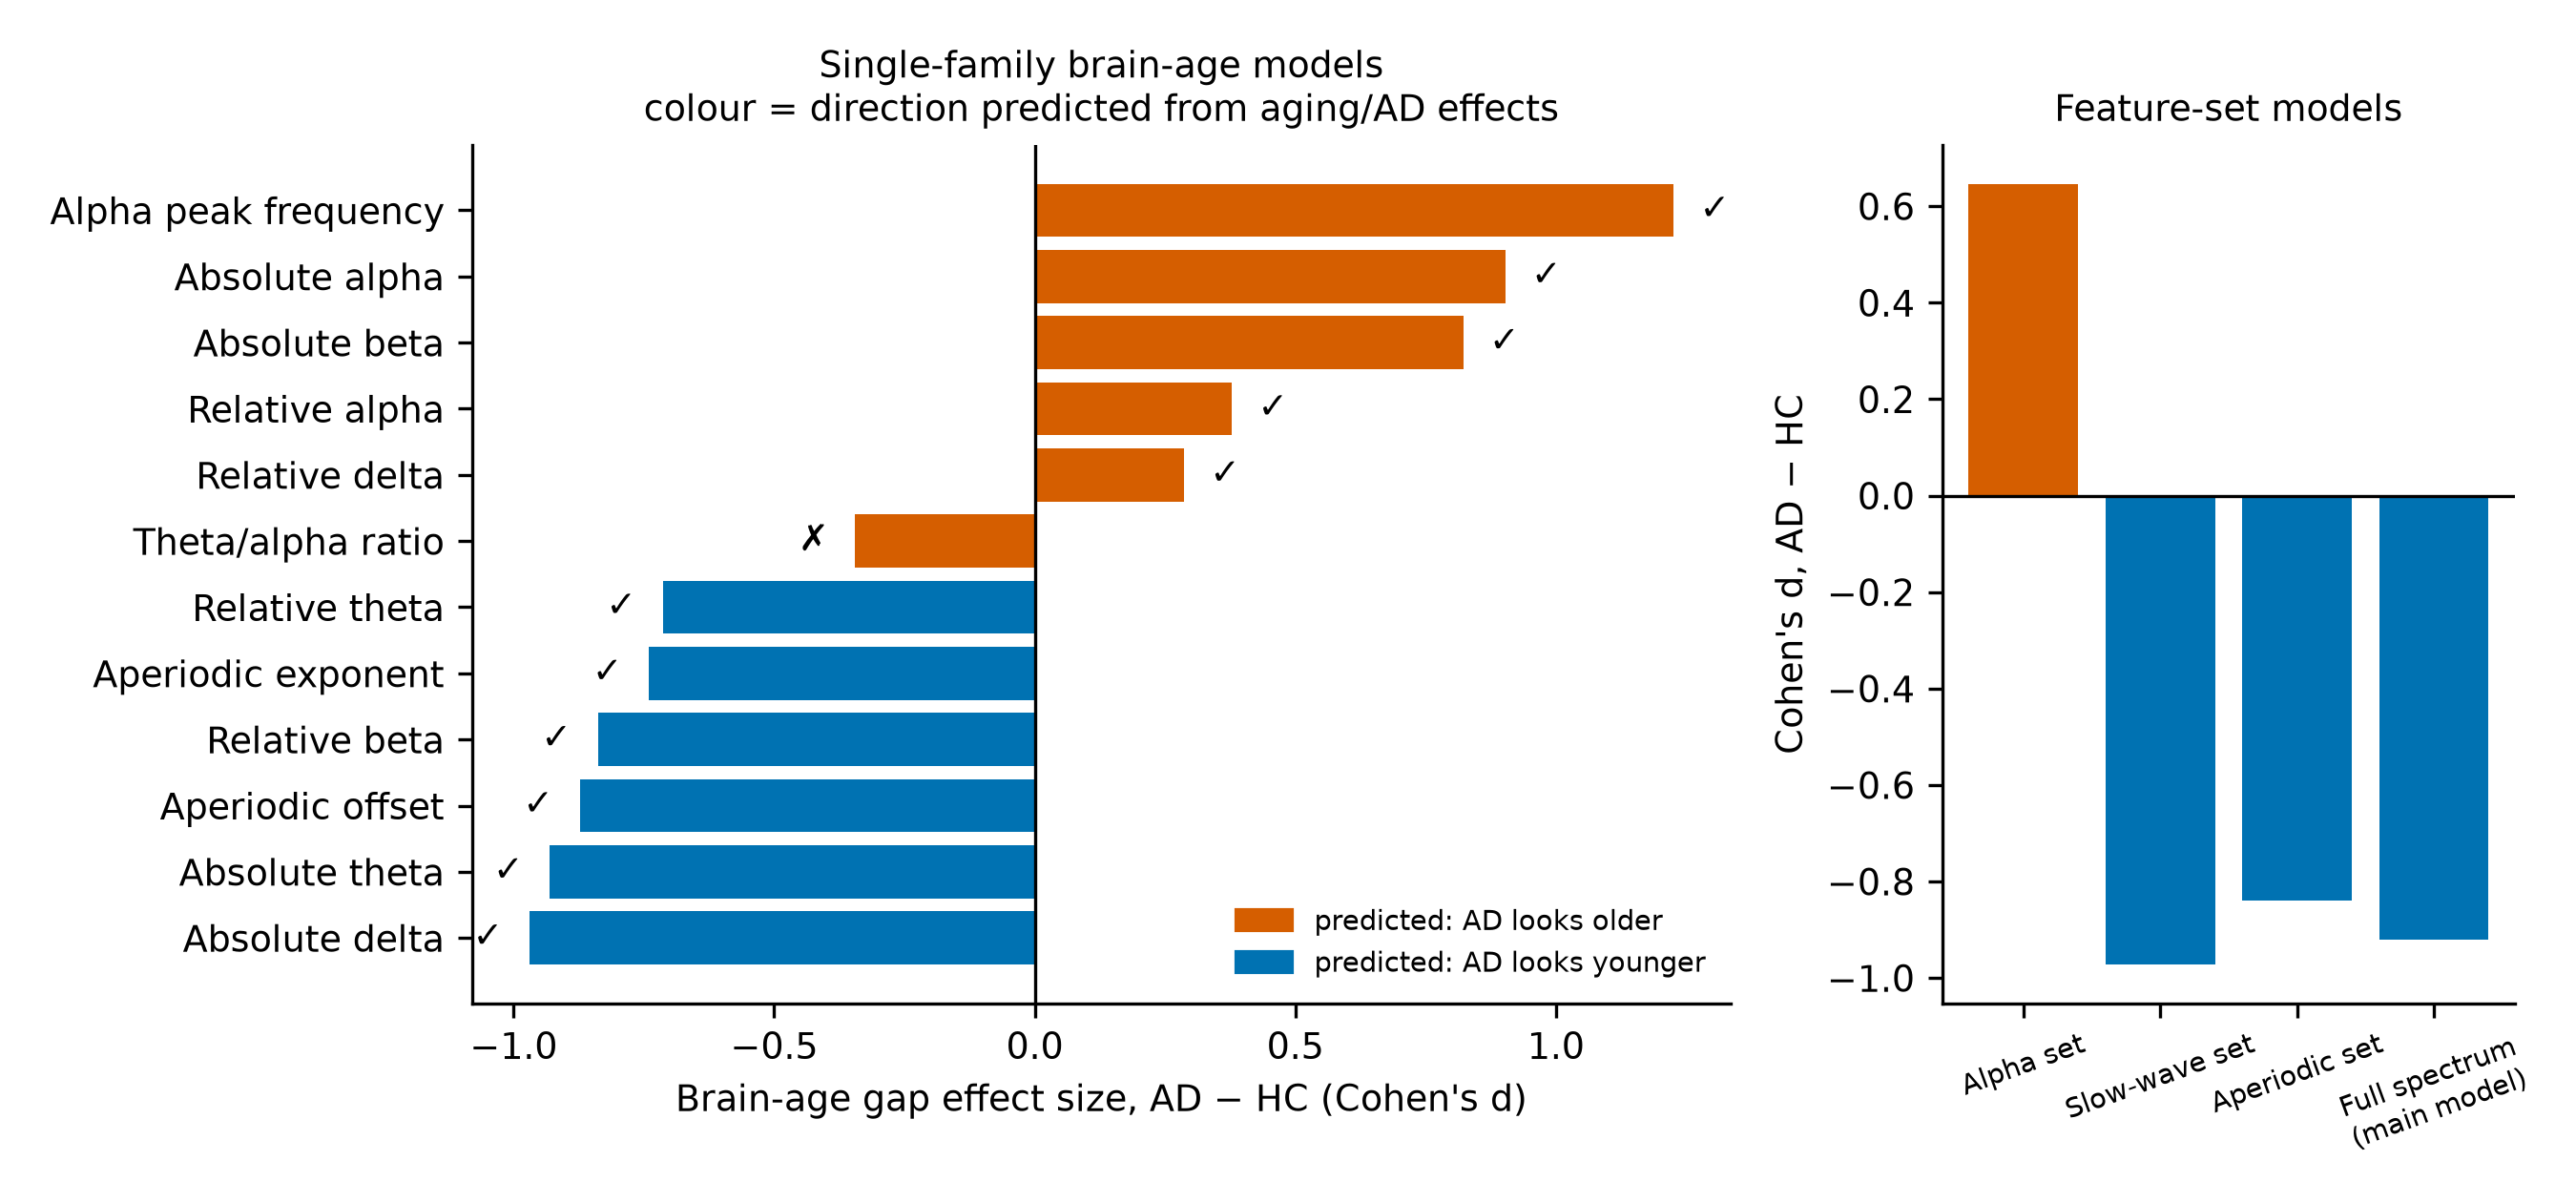
\includegraphics[width=0.85\textwidth]{fig_feature_family_brainage.png}
\caption{Feature-dependence of the brain-age gap. Left: single-family models, coloured by the direction predicted before the analysis (\checkmark{} = observed direction agrees). Right: feature-set models.}
\label{fig:fam}
\end{figure*}

\subsection{Q3: Normative deviation outperforms the scalar BAG}
The multivariate deviation score separated AD from HC with $d=\normD{}$ \normDci{} and AUC \normAUC{} (cross-validated \normAUCcv{}; age/sex-adjusted \normAdjP{}), compared with BAG AUC \bagAUC{}. It was not AD-specific: FTD also deviated ($d=\normFTDd{}$, \normFTDp{}), and AD did not differ from FTD (\normADFTDp{}). AD showed elevated slow-wave and aperiodic $z$-scores and reduced alpha, beta and alpha-peak $z$-scores (Fig.~\ref{fig:norm}).

\begin{figure*}[t]
\centering
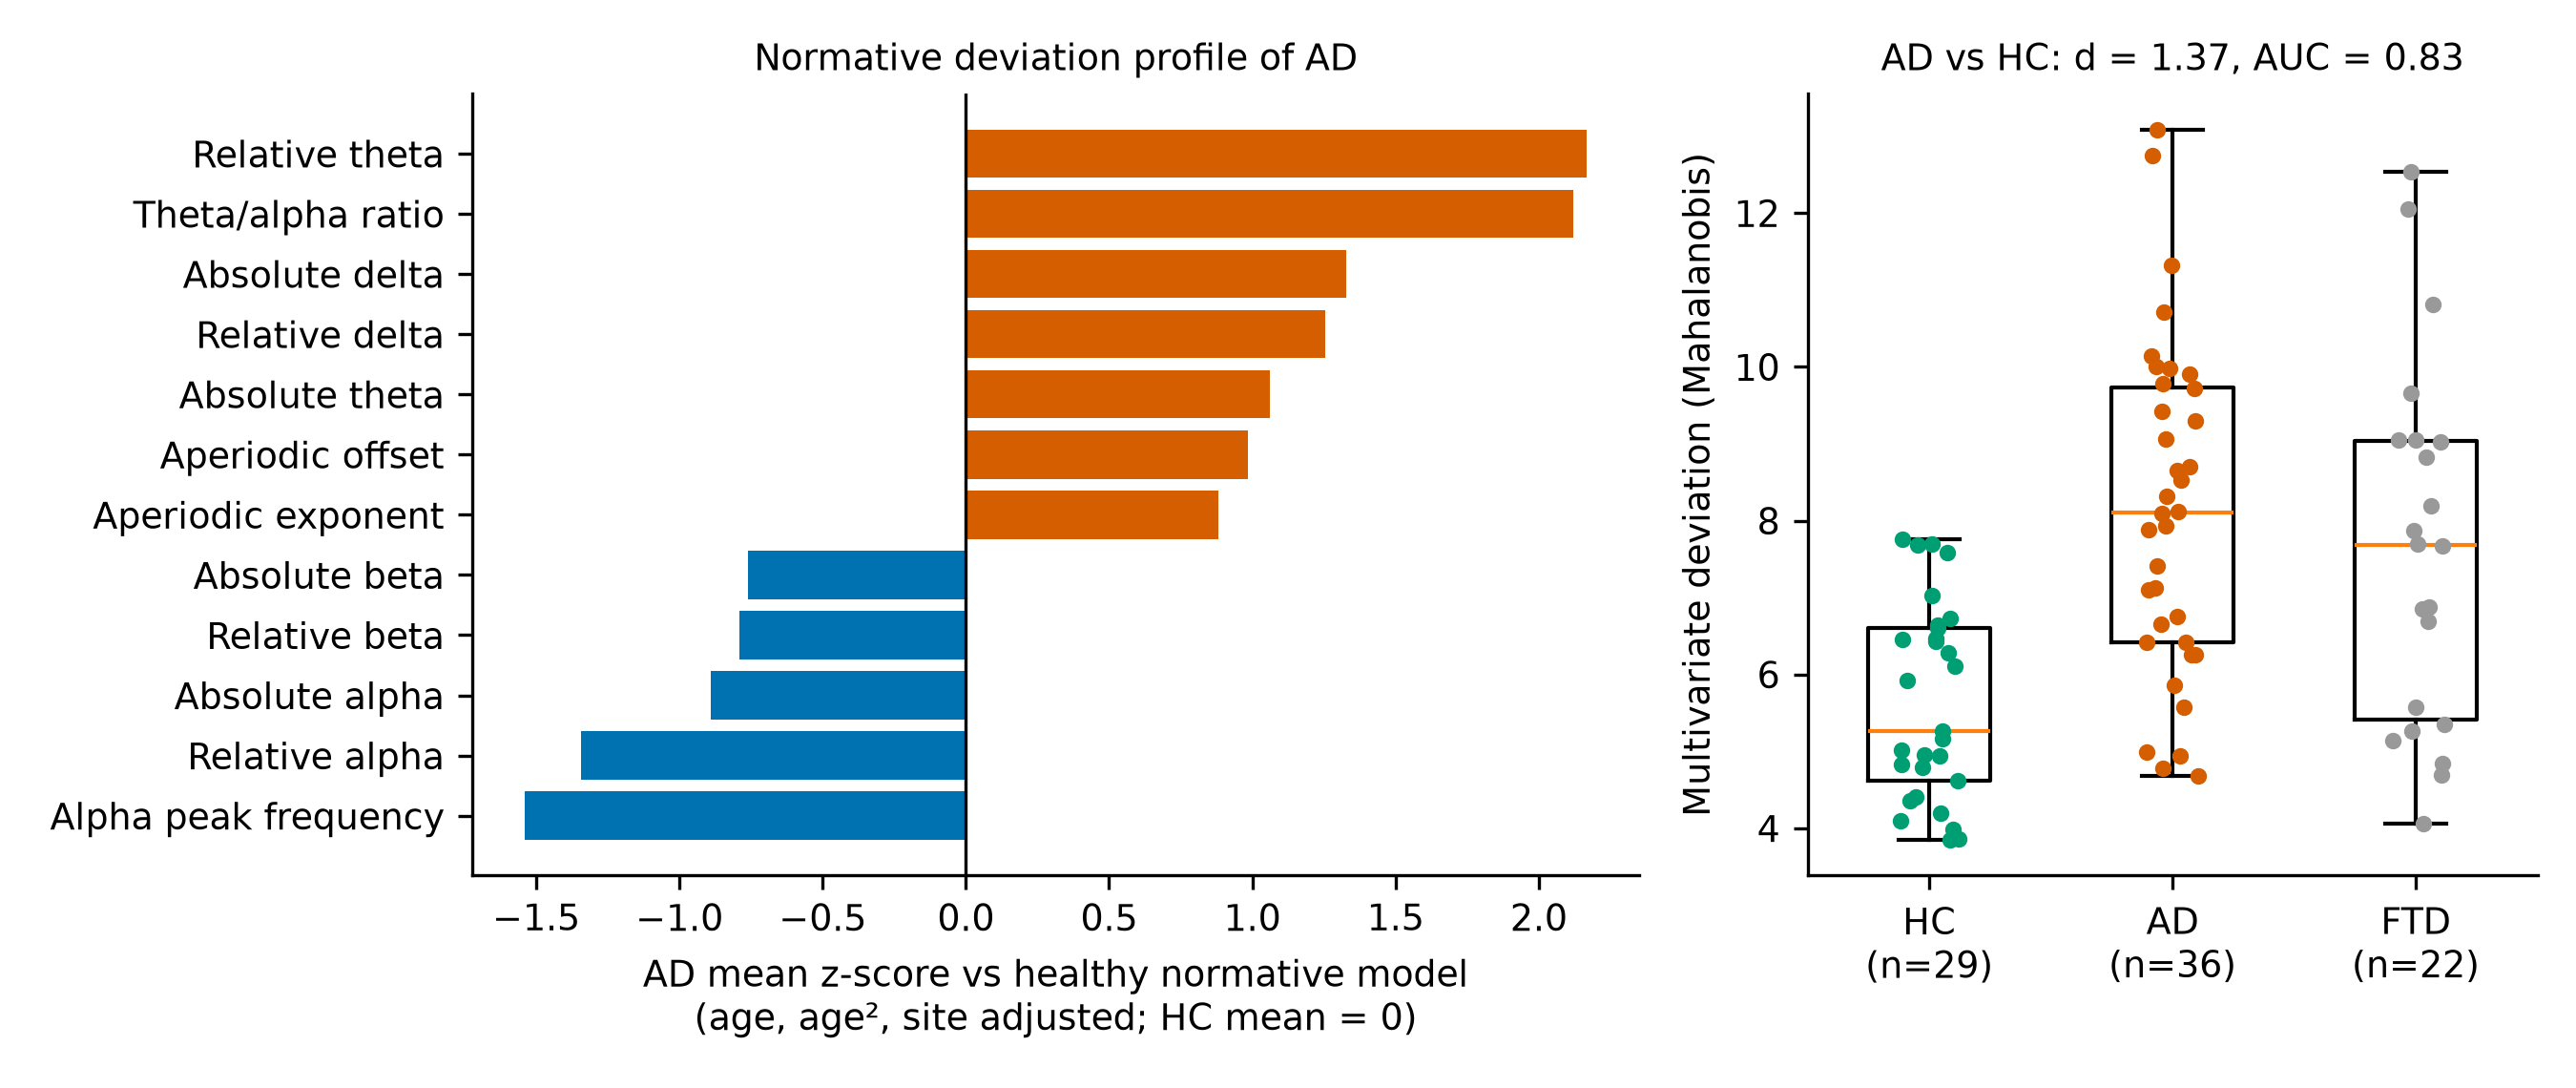
\includegraphics[width=0.85\textwidth]{fig_normative_deviation.png}
\caption{Normative deviation. Left: AD mean $z$ per feature family relative to an age-, age$^2$- and site-adjusted healthy reference. Right: multivariate deviation by group (HC scored leave-one-out).}
\label{fig:norm}
\end{figure*}

\subsection{Q4: Classification, stacking and explainability}
The CNN reached a mean AUC of \cnnAUC{} over three seeds (range \cnnAUClo{}--\cnnAUChi{}; accuracy \cnnAcc{}). For the primary seed: AUC \cnnPrimAUC{} \cnnPrimAUCci{}, PR-AUC \cnnPRAUC{}, balanced accuracy \cnnBalAcc{}, Brier \cnnBrier{}, ECE \cnnECE{}; permutation \cnnPermP{} ($N=\cnnPermN{}$). On identical folds, EEGNet (\aucEEGNet{}), random forest (\aucRF{}), SVM (\aucSVM{}) and logistic regression (\aucLR{}) were statistically indistinguishable from the CNN (\holmText{}; Table~\ref{tab:models}, Fig.~\ref{fig:forest}). Performance was similar for women and men (AUC \subFemAUC{} vs.\ \subMaleAUC{}) and across age tertiles (\subAgeLo{}--\subAgeHi{}). In fully nested stacking, the CNN alone gave AUC \nestCnnAUC{}, BAG alone \nestBagAUC{} (vs.\ chance \nestBagP{}) and CNN+BAG \nestCombAUC{} ($\Delta=\nestDiff{}$, \nestDiffCI{}, \nestDiffP{}). Ablations (three seeds each) gave mean AUCs from \ablMin{} to \ablFull{} (full model \ablFull{}; 8 channels \ablEight{}; 40\% of epochs \ablSixty{}; no time axis \ablNoTime{}). The three-class balanced accuracy was \mcBalAcc{} (random forest \mcRFBalAcc{}).

\begin{table*}[t]
\centering
\caption{AD vs.\ HC, out-of-fold on identical subject folds ($n=65$), with 95\% bootstrap CIs for AUC}
\label{tab:models}
\begin{tabular}{lcccccc}
\toprule
Model & AUC [95\% CI] & PR-AUC & Bal.\ acc. & Sens. & Spec. & Brier \\
\midrule
\tableinput{table_models.tex}
\bottomrule
\end{tabular}
\end{table*}

\begin{figure}[t]
\centering
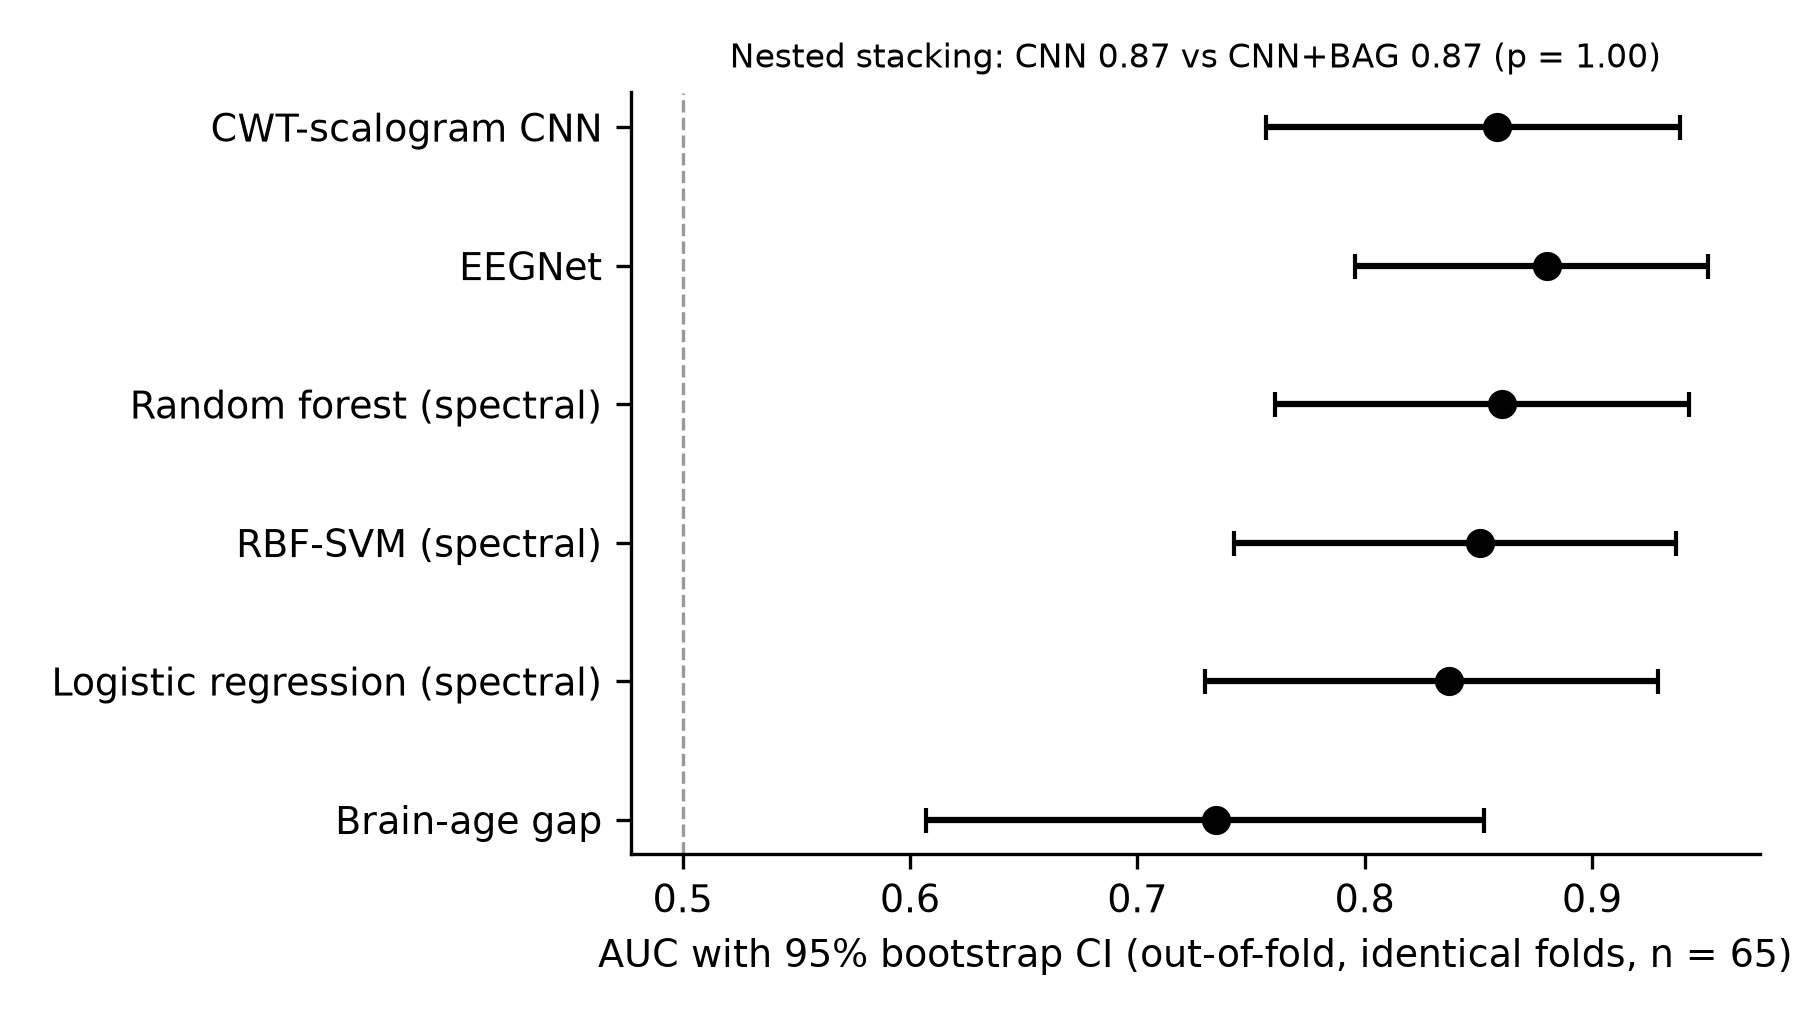
\includegraphics[width=0.95\columnwidth]{fig_model_forest.png}
\caption{AUC with 95\% CIs on identical folds; nested-stacking comparison in the title.}
\label{fig:forest}
\end{figure}

Out-of-fold Grad-CAM profiles were stable across seeds ($r$ \gcStabLo{}--\gcStabHi{}) and emphasized theta (\gcTheta{}), alpha (\gcAlpha{}) and beta (\gcBeta{}) relative to average. Occlusion, however, showed that the models depended mostly on beta (AUC drop \occBeta{}) and delta (\occDelta{}), little on alpha (\occAlpha{}) and not on theta (\occTheta{}). Spatially, occipital (\occOccipital{}), frontal (\occFrontal{}) and temporal (\occTemporal{}) regions mattered most (Fig.~\ref{fig:xai}). Grad-CAM importance therefore did not identify the information the model needs.

\begin{figure}[t]
\centering
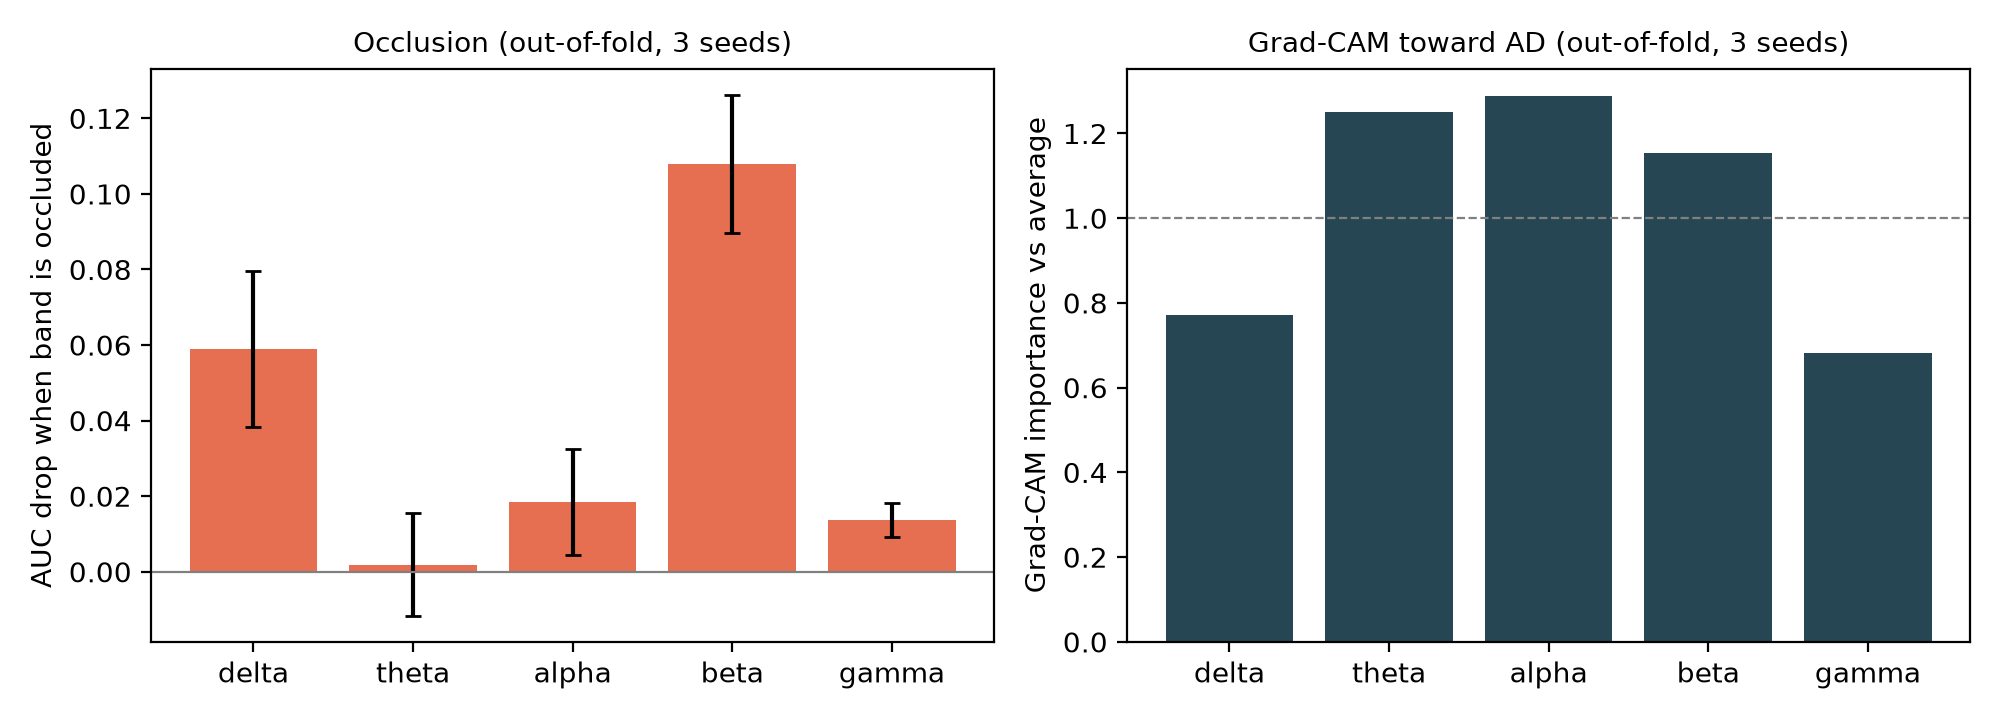
\includegraphics[width=\columnwidth]{xai_occlusion_vs_gradcam.png}
\caption{Explanation validation: AUC drop when a band is occluded (left) vs.\ Grad-CAM band importance (right), out-of-fold, three seeds.}
\label{fig:xai}
\end{figure}

% =====================================================================
\section{Discussion}
\emph{Why the sign depends on the features.} Healthy aging and AD share alpha slowing, but they move absolute slow-wave power, beta power and the aperiodic component in opposite directions~\cite{babiloni2020}. A brain-age model is a projection of the EEG onto the healthy-aging axis. Its sign in AD is therefore determined by which features dominate that projection. Our pre-registered family analysis confirmed this (\famAgree{}), and an alpha-only model reproduced the positive gaps of~\cite{otero2026}. Positive and negative EEG BAGs in AD are thus not contradictory findings but different projections of the same deviation. The multivariate normative score, which does not force the deviation onto an age axis, captured it better (AUC \normAUC{}). This supports reporting EEG abnormality in AD as a normative deviation rather than a ``brain age''.

\emph{Alternative explanations.} We controlled for leakage, bias correction, model choice, sex, age, epoch count, artifact threshold, ICA and training age range, and the effect remained. The external healthy cohort argues against a site artifact of older healthy brains. Because the scalar BAG is not associated with MMSE, and because FTD shows a similar multivariate deviation, we do not claim BAG as a severity or AD-specific biomarker. Sex is a relevant moderator: within HC, women appeared younger. Its residual confounding cannot be excluded with $n=65$.

\emph{Classification and explanations.} The CNN performed comparably to well-tuned spectral baselines and EEGNet, and to published subject-independent results on this dataset~\cite{miltiadous2021,miltiadous2023dice}. We do not claim superiority. Grad-CAM was stable but not faithful: occluding theta, emphasized by Grad-CAM, did not reduce performance, consistent with redundancy across bands. Stability of explanations should not be mistaken for validity.

\emph{Limitations.} The clinical cohort is small and comes from a single site; there is no independent AD cohort, because access to CAUEEG and BrainLat is pending. MMSE is the only clinical scale, and there are no MCI subjects. LEMON ages are binned. Our features are sensor-space and average-referenced over 19 channels, whereas~\cite{otero2026} used source-space alpha; the qualitative agreement of our alpha-only model with their result does not establish quantitative equivalence. Several model variants and the CNN early-stopping criterion were chosen after earlier results were visible; all are disclosed and reported as sensitivity analyses.

% =====================================================================
\section{Conclusion}
A full-spectrum resting-state EEG brain-age model trained on healthy adults places AD \emph{younger}, not older, and this result survives extensive leakage control. Yet the sign of the gap is a property of the feature set: alpha-based models place AD older. AD EEG is better characterized as a multivariate deviation from normative aging. Independent AD cohorts with harmonized feature sets are required before clinical use.

\section*{Data and Code Availability}
OpenNeuro ds004504 and ds005385 and MPI-LEMON are public. All code, saved models, out-of-fold predictions, fold assignments, seeds, audit reports and the scripts generating every number in this paper are in the project repository (branch \texttt{q1-upgrade}).

\section*{Ethics Statement}
Only publicly available, de-identified data collected under the original studies' approvals were used.

\section*{Declaration of Generative AI Use}
The authors used Claude (Anthropic) to assist with code development, analysis and manuscript drafting. The authors verified all code, results and references and take full responsibility for the content. \textcolor{red}{[Authors: confirm the wording against the target journal's policy.]}

\section*{Author Contributions}
\textcolor{red}{[Authors to provide individual CRediT roles; not invented here.]}

\section*{Funding and Conflicts of Interest}
\textcolor{red}{[Authors to confirm: no external funding.]} The authors declare no conflict of interest.

\section*{Acknowledgment}
We thank Prof.~Manasa (B.\,M.\,S. College of Engineering) for supervision, and the investigators of ds004504, ds005385 and MPI-LEMON for sharing their data.

\bibliographystyle{IEEEtran}
\bibliography{refs}
\end{document}
